\section{Flutter}

\textit{Flutter} ist ein von \textbf{Google} entwickeltes \textit{User-Interface-Framework} zur
Entwicklung plattformunabhängiger Apps sowohl für Web, Desktop als auch Mobile.

Neben der Möglichkeit Apps für verschiedene System erstellen zu können, ohne etwas mehrfach programmieren
zu müssen, bietet Flutter auch einen integrierten Widget-Katalog voll vorgefertigter UI-Elemente.\\
Diese können nach Belieben verwendet, umgestaltet und miteinander kombiniert werden.

Flutter bietet hiermit auch Personen mit weniger Erfahrung auf dem Gebiet der Software-Entwicklung
die Möglichkeit, relativ einfach eigene Apps zu entwickeln.

\subsection{Was macht Flutter besonders?}

\subsubsection{Design-Architektur}

Der Clou hinter Flutter steckt in seiner Architektur und Design-Struktur, denn in diesem Framework ist \textbf{alles} ein Widget,
von der eigentlichen App bis hin zum einfachen Text.

\begin{figure}[H]
    \begin{center}
        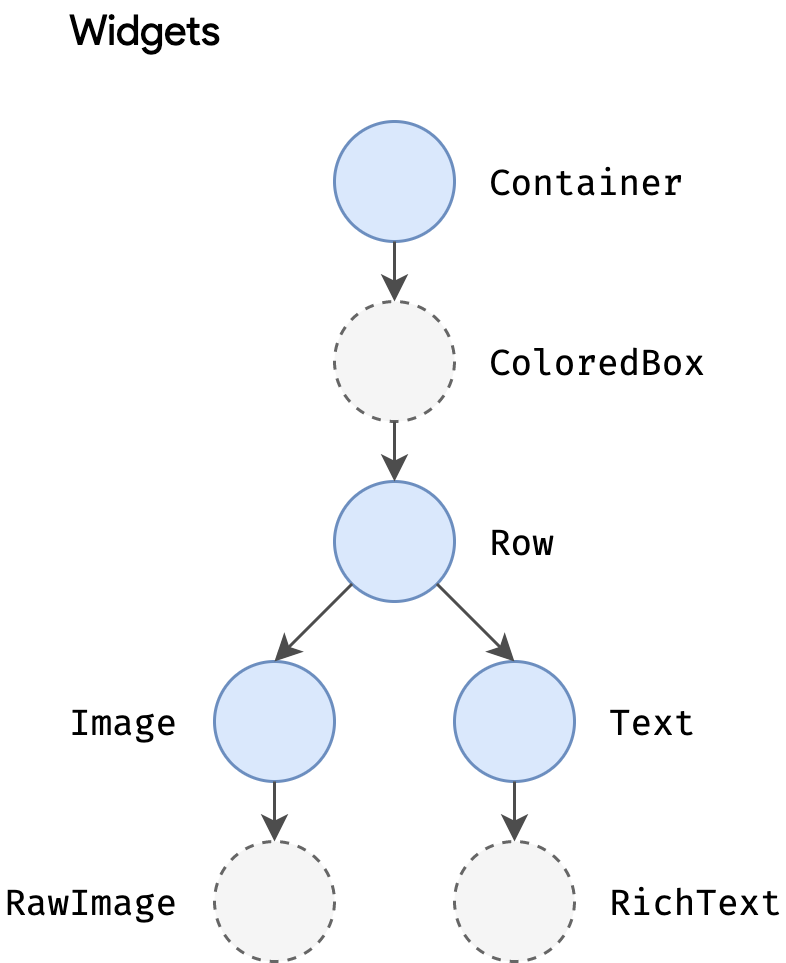
\includegraphics[width=0.5\textwidth]{images/Flutter/design-structure.png}
        \caption{Design-Struktur und Widget-Aufbau von Flutter}
        \cite{flutterDesignArchitecture}
        % https://flutter.dev/docs/resources/architectural-overview
    \end{center}
\end{figure}

Der Aufbau und das Erstellen eines User-Interfaces mithilfe von Flutter erfolgt in erster Linie
durch das Kombinieren, Zusammenbauen und Verschachteln von Widgets.
Abhängig von ihrem Zustand (\textit{Widget-State}) und ihren Attributen beschreiben jene Widgets, wie das entsprechende
View zur Laufzeit aussehen wird.

Ändert sich der Zustand eines Widgets, wird es erneut aufgebaut und gerendert. Die Flutter-Engine 
vergleicht dabei vorherige Zustände mit der neuen Änderung und rendert nur jene Widgets neu, die
sich auch wirklich verändert haben.

Auf diesem Wege kann der Renderprozess von Widgets so schnell wie möglich durchlaufen werden, wodurch
auch die Performance der App gesteigert wird.

Auf diesem Prinzip baut auch Flutters \textit{Hot-Reload}-Funktion bei der Entwicklung auf. Mithilfe dieser
können Veränderungen an der App in wenigen Augenblicken auf den Emulator übertragen werden, ohne, dass es einen
Neustart der App bedingt.\\
So können selbst die kleinsten Veränderungen schnell ausprobiert und getestet werden, ohne einen erneuten Build von Grund auf
zu benötigen.

\subsubsection{Plattformunabhängigkeit}

Mithlfe von Flutter können Apps unabhängig ihrer Plattform entwickelt werden, das heißt, dass eine Code-Base
sowohl als Android-App und iOS-App als auch als Web-App deployed werden kann.\\
Neben den enormen Zeitersparnissen werden ebenso die nötigen Kenntnisse zweier Programmiersprachen, beispielsweise
\textit{Kotlin} für Android und \textit{Swift} für iOS, auf \textbf{Dart} reduziert.

Unter anderem wird dies durch den oben erwähnten Widget-Katalog erzielt. Dieser bietet zwei Varianten
von Widgets an, einerseits die \textit{Material Components} für Android, andererseits die \textit{Cupertino Components}
für iOS.\\
Das jeweilige Widget-Paket passt sich adaptiv an das Design des entsprechenden Betriebssystem an, um ein einen möglichst
geringen UI-Kontrast zwischen App und dem Rest des Betriebssystems zu garantieren.

% Kombination von Material & Cupertino oder Default mit Custom Scrolls.

\begin{figure}[H]
    \begin{center}
        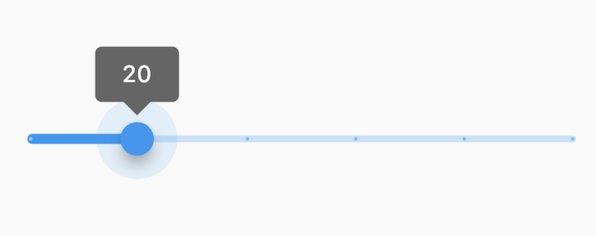
\includegraphics[width=0.5\textwidth]{images/Flutter/material-slider.png}
        \caption{Slider-Widget im Material-Design für Android}
        \cite{flutterMaterialSlider}
        % https://flutter.github.io/assets-for-api-docs/assets/material/slider.png
    \end{center}
\end{figure}

\begin{figure}[H]
    \begin{center}
        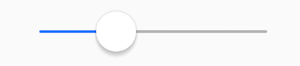
\includegraphics[width=0.5\textwidth]{images/Flutter/cupertino-slider.png}
        \caption{Slider-Widget im Cupertino-Design für iOS}
        \cite{flutterCupertinoSlider}
        % https://flutter.dev/images/widget-catalog/cupertino-slider.png
    \end{center}
\end{figure}

\subsection{Layoutting in Flutter}

Den Kern von Flutters Layout-System bilden, wie bereits erwähnt, die einzelnen Widgets, deren Attribute und ihr
kaskadierendes Verhalten zueinander.

\begin{figure}[H]
    \begin{center}
        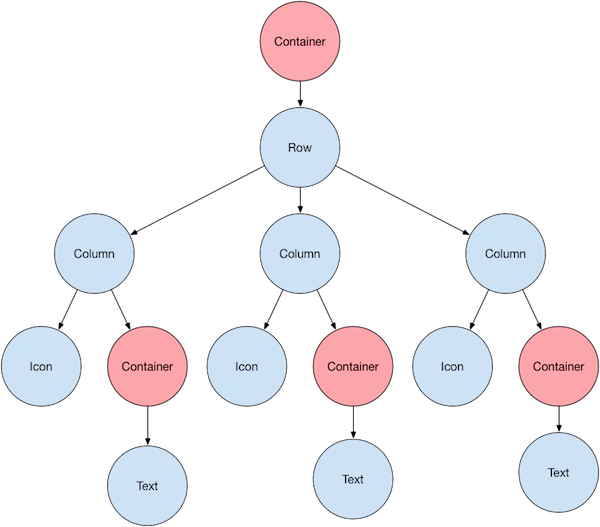
\includegraphics[width=0.65\textwidth]{images/Flutter/widget-tree.png}
        \caption{Widget-Tree für ein beispielhaftes Layout}
        % https://flutter.dev/images/widget-catalog/cupertino-slider.png
        \cite{flutterWidgetTree}
    \end{center}
\end{figure}

Ähnlich zu anderen Frameworks wie beispielsweise \textit{Bootstrap 4}
können unter Einsatz von bekannten Standard-Widgets wie Containern, Rows und Columns
bereits simple Layouts erstellt werden.\\

Ein Widget wird in Flutter mithilfe des entsprechenden Objekt-Konstruktors
an der gewünschten Stelle erzeugt und mit entsprechenden Attributen befüllt.

\begin{lstlisting}
...
new Container(
    height: 280.0,
    width: 400.0,
    padding: new EdgeInsets.only(top: 10.0),
    child: new Text('Sokka is awesome!')
),
...
\end{lstlisting}

Hiermit wird ein neues Container-Widget mit 280 Pixeln Höhe,
400 Pixeln Breite, einem Top-Padding von zehn Pixeln und einem Text als
Kind-Widget erzeugt.

Wie bereits erwähnt können durch das Kaskadieren unterschiedlicher Widgets
relativ einfach komplexe UI-Strukturen erzeugt werden.\\
Hierfür müssen lediglich die weiteren / inneren Widgets dem 
\textit{child}- bzw. \textit{children}- Property übergeben werden.
\pagebreak
\begin{lstlisting}
...
new Container(
    child: new Row(
        children: <Widget>[
            new Icon(
                Icons.ac_unit,
                color: Colors.white,
            ),
            new Text(
                'Sokka is awesome!',
                color: Colors.white,
            ),
            new Container(
                child: new Image(...)
            ),
        ],
    ),
),
...
\end{lstlisting}

% https://flutter.dev/assets/ui/layout/sample-flutter-layout-46c76f6ab08f94fa4204469dbcf6548a968052af102ae5a1ae3c78bc24e0d915.png
% https://flutter.dev/docs/development/ui/layout

\subsection{Rendern von Widgets}

\subsection{Interaktivität von Widgets}

\subsection{App-States und ephimerale States}

\subsection{Navigation und Routing durch die App}













